\documentclass{oci}
\usepackage[utf8]{inputenc}
\usepackage{lipsum}
\usepackage{calc}
\usepackage{tikz}
\usepackage{ifthen}
\usetikzlibrary{matrix}

\title{Roberto el constructor}

\begin{document}
\begin{problemDescription}
  A Roberto le han encargado construir un nuevo edificio.
  En un principio todo parecía ser una construcción rutinaria hasta que Roberto vio el plano
  del terreno y se dio cuenta de que este es totalmente irregular.

  El plano describe el terreno como una matriz de enteros de tamaño $H\times W$
  ($H$ filas y $W$ columnas).
  Cada elemento en la matriz representa la altura del terreno en esa posición.
  El nuevo edificio debe construirse sobre una submatriz de tamaño $M\times N$.
  Antes de construirlo, Roberto tiene que nivelar la submatriz sobre la cual se construirá.
  El costo de nivelación de una submatriz es igual a la diferencia entre las alturas de la celda
  más alta y la más baja en la submatriz.

  A continuación se muestra un ejemplo para un terreno de tamaño $4\times 5$ donde se ha marcado
  una submatriz de tamaño $3\times 2$.
  Para esta submatriz la celda de menor altura tiene altura 8 y la de mayor altura tiene altura 80.
  Por lo tanto, el costo de nivelación de esta submatriz es $80 - 8=72$.

  \begin{center}
    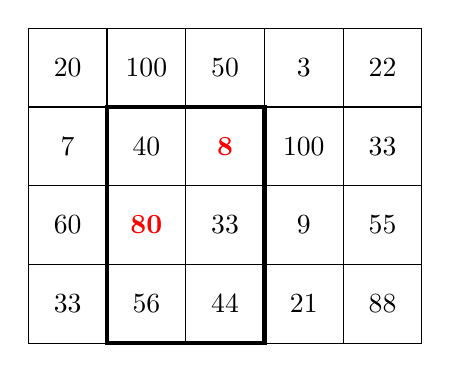
\begin{tikzpicture}
      \edef\H{4}
      \edef\W{5}
      \draw[step=1cm, thin] (0, 0) grid (\W, \H);
      \draw[ultra thick] (1, 0) rectangle (3, 3);
      % \foreach \y in {0,..., 3} {
      %   \node[font=\footnotesize] at (-0.3, \H - \y - 0.5) {\y};
      % }
      % \foreach \x in {0,..., 4} {
      %   \node[font=\footnotesize] at (\x + 0.5, \H + 0.3) {\x};
      % }
      \foreach \v [count=\i] in { 20, 100, 50,   3, 22
                                ,  7,  40,  8, 100, 33
                                , 60,  80, 33,   9, 55
                                , 33,  56, 44,  21, 88
                                } {
        \pgfmathparse{mod(\i - 1, \W)}
        \edef\x{\pgfmathresult}
        \pgfmathparse{int((\i - 1)/\W)}
        \edef\y{\pgfmathresult}
        \ifthenelse{\i = 8 \OR \i = 12}{
          \node[text=red, font=\bf] at (\x + 0.5, \H - \y - 0.5) {\v};
        }{
          \node at (\x + 0.5, \H - \y - 0.5) {\v};
        }
      }
    \end{tikzpicture}
  \end{center}

  Roberto desea encontrar una submatriz de forma que el costo de nivelación sea mínimo.
  En el ejemplo anterior no hay ninguna otra submatriz de tamaño $3\times 2$ con un costo de
  nivelación menor y por lo tanto el costo mínimo para este tamaño de submatriz es 72.
  % ?`Podrías ayudarlo?
\end{problemDescription}

\begin{inputDescription}
  La primera línea de la entrada contiene cuatro enteros $H, W, M$ y $N$
  ($0 < M \leq H\leq 1000, 0 < N \leq W \leq 1000$).
  Estos enteros corresponden respectivamente al alto y ancho de la matriz describiendo el terreno,
  y al alto y ancho de la submatriz donde se debe construir el edificio.
  Las siguientes $H$ líneas describen la matriz que representa el terreno.
  Cada línea contiene $W$ enteros entre 0 y 1000.
  El $j$-ésimo entero en la línea $i$-ésima corresponde al entero en la fila $i$-ésima y
  columna $j$-ésima de la matriz.
\end{inputDescription}

\begin{outputDescription}
  La salida debe contener un único entero correspondiente al costo de nivelación de la submatriz
  de tamaño $M\times N$ de menor costo.
\end{outputDescription}


\begin{scoreDescription}
  \subtask{10}
  Se probarán varios casos en que $H=W=M=N$.
  \subtask{15}
  Se probarán varios casos en que $M=N$ y $M\leq 5$.
  \subtask{30}
  Se probarán varios casos en que $H=1$ y $M=1$.
  \subtask{45}
  Se probarán varios casos sin restricciones adicionales.
\end{scoreDescription}

\begin{sampleDescription}
\sampleIO{sample-1}
\sampleIO{sample-2}
\sampleIO{sample-3}
\end{sampleDescription}

\end{document}
